\section{Data and Feature Vectors}


\noindent Right now we have 1500 characteristic polymeric systems (chemicals that are built from repeated units, like plastic/rubber/Nylon) in our tentative training set. These systems are made up from 7 different major building blocks, (phenyl, furan, vinyl, acetylene, pyrrole, pyridine, and ketone), and 7 minor building blocks, (Hydrogen, methyl, hydroxyl, methoxy, carbenyl, cyano, and amine). Some visualized polymer structures are shown in Fig ~\ref{furan}. They are divided into one group that consists of Oxygen (O) and another group that consists of Nitrogen (N) for chemical analysis. Quantum chemistry software package \textit{Gaussian} \cite{gaussian} is applied to compute HOMO, LUMO and band gap at three different DFT levels, namely B3LYP, CAM-B3LYP, and M06HF. Fig ~\ref{orbital} shows the an example calculated HOMO and LUMO. These 3 theories have been widely tested in chemical research, and they lead to slightly different numerical results. In addition, each of these methods defines an energetically favored geometrical structure for each of the molecules; these structures are slightly different, and it is reasonable to think that each of them contains some information. Along with the initial non-optimized geometrical structure, we have 4 types of structures; combining with the aforementioned 3 DFT theories, we have essentially obtained 12 data sets that contain slightly different information, yielding $\sim12000$ unique data points. \\

\begin{figure}[hb]
\begin{center}
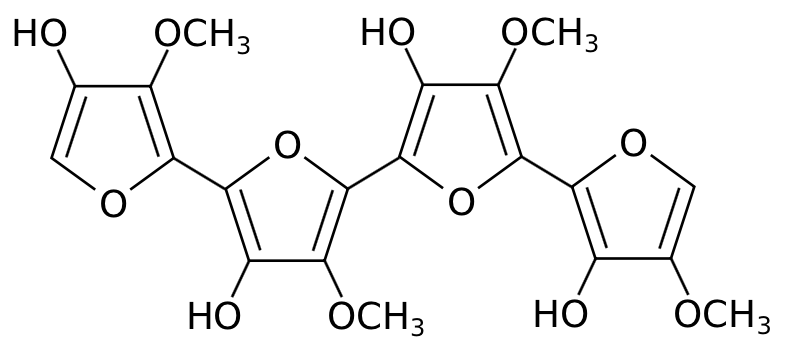
\includegraphics [width=.1\textwidth]{furan.png}
\caption{example polymer structure of furans}\label{furan}
\end{center}
\end{figure}

\begin{figure}[hb]
\begin{center}
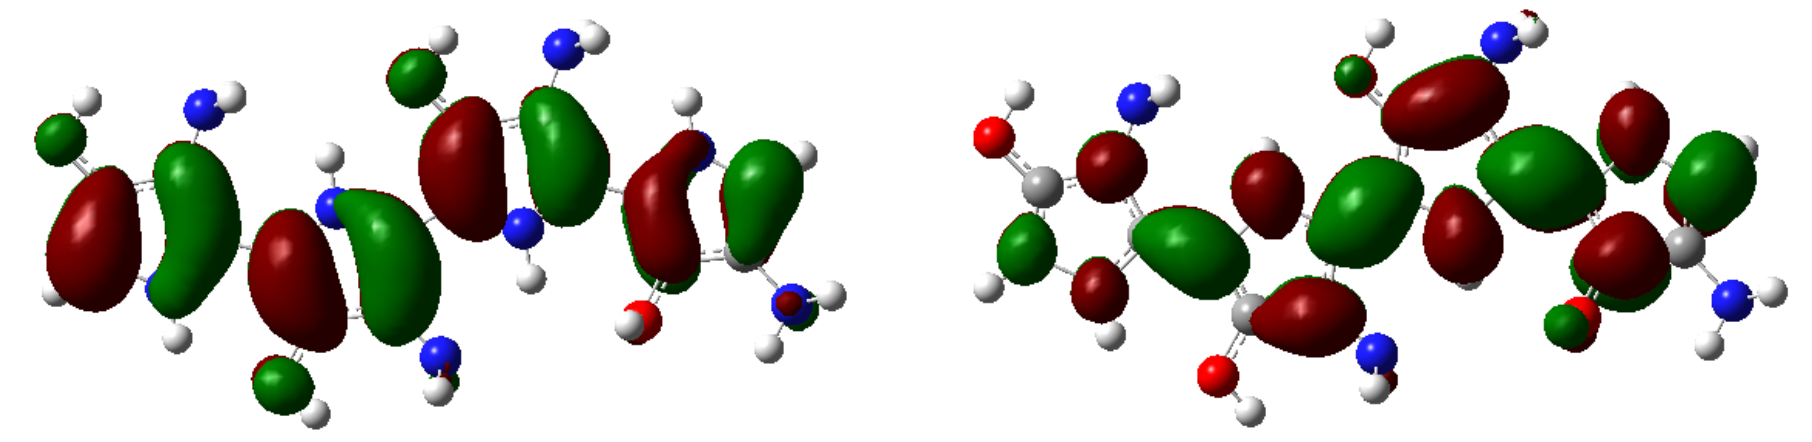
\includegraphics [width=1\textwidth]{orbital.png}
\caption{Example HOMO (left) and LUMO (right) orbitals}\label{orbital}
\end{center}
\end{figure}

The following part shows how we extract 11 types of feature vectors from each structure based on chemical intuition:

\begin{enumerate}
\item \textbf{Null}: An empty list that serves as the worst result to compare against. This feature vector also is used to compare the amount of error that is contained implicitly in each of the different data sets.

\item \textbf{Binary}: It creates a simple boolean feature vector based on whether or not a building block exists in the structure. Mostly speaking, we only consider the existence of aryl-group and r-group. For example, it turns each building block into 1 or 0 in Fig ~\ref{binary feat}

\begin{figure}[hb]
\begin{center}
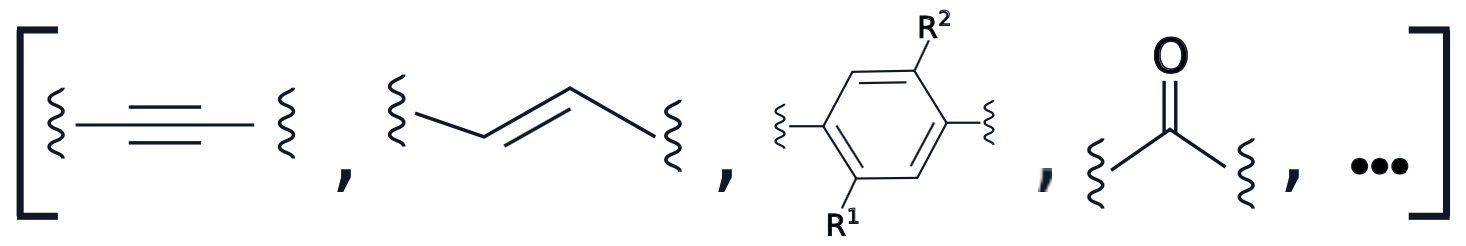
\includegraphics [width=1\textwidth]{binaryfeat.png}
\caption{Example binary feature vector}\label{binaryfeat}
\end{center}
\end{figure}

\item \textbf{Flip Binary}: This is similar to the binary feature vector, except that for each aryl group that appears in the structure, it takes into account whether or not the ring was rotated 180 along the connecting bond between the two units. When dealing with conjugated systems, like we have, the rotations can be a significant effect. This vector takes that into account by adding an extra binary feature for each link in the chain.

\item \textbf{Decay}: This feature vector makes the approximation that the relation between all of the atoms/structures within the molecule have some sort of a intrinsic decay, (atoms infinitely far apart should not influence each other). For this, the first aryl group in the chain is considered the zero point (influence of 1), and all the subsequent aryl groups influences are defined by a decay function $\sum_{i} (Ad_{i}^{-H})^{p}$, where $A$, $H$, $p$ are constant factors to determine rate of decay, $d_{i}$ is the distance from the $i$th group. This feature also has the added benefit that it has $O(1)$ space requirements compared to the normal binary feature vector which is $O(N)$ where $N$ is the number of aryl groups.

\item \textbf{Centered Decay}: This feature vector takes the same approach as the decay feature vector with the addition that it does the decay from the center of the structure using a radial distance.

\item \textbf{Signed Centered Decay}: This works similar to the centered decay feature vector with the addition that it takes into account the side of the center that the rings are on instead of just looking at the magnitude of the distance.

\item \textbf{Gaussian Decay}: This feature vector works the exact same as the normal decay feature vector with the exception that it uses a Gaussian distribution for the decay. This was picked because looking at the PCA components for the parts of the structure and their relative influence as they were farther in the name from the start in the binary feature vector.

\begin{figure}[H]
\begin{center}
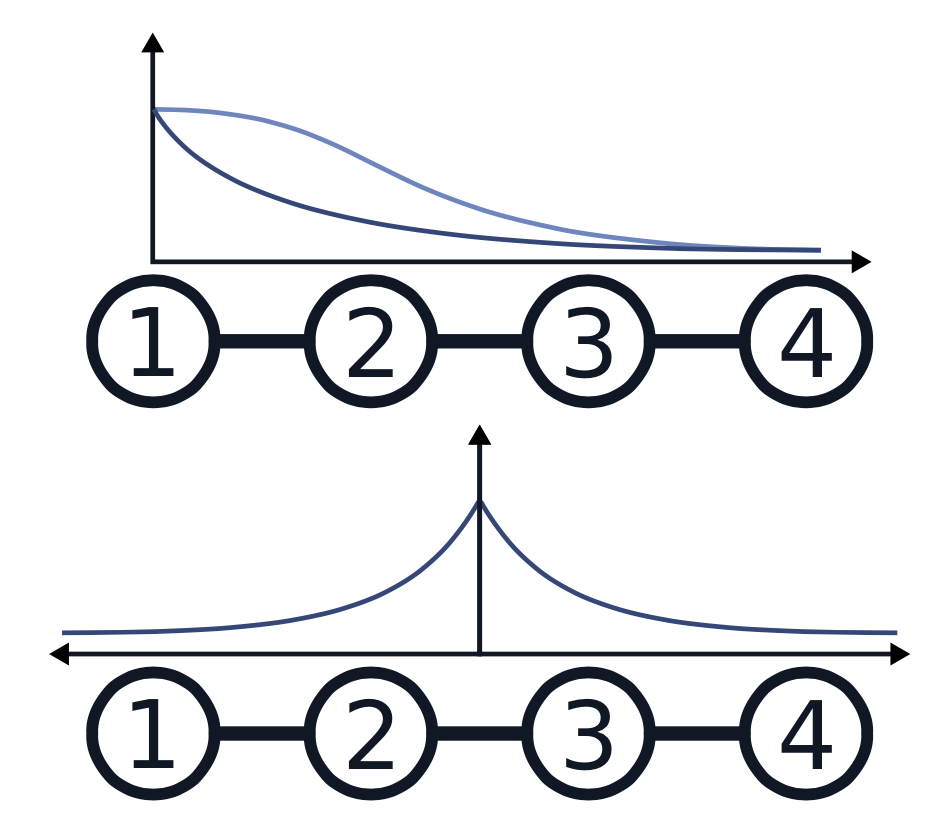
\includegraphics [width=0.4\textwidth]{decay.png}
\caption{Example decay feature}\label{decay}
\end{center}
\end{figure}

\item \textbf{Coulomb}: This feature vector is based on a distance matrix between all of the atoms in the structure with each element multiplied by the number of protons in each of atom in the pair. The diagonal is $0.5 \times N_{photons}^{2.4}$. The exponent comes from a fit.

\item \textbf{PCA Coulomb}: This feature vector takes the feature matrix from coulomb feature and does Principal Component Analysis on it to extract the N most influential dimensions. The goal of this is to reduce the size of the feature vector which can reduce overfitting, and most importantly dramatically reduce running time. In principal, the number of dimensions used should correspond to at least $95\% $ of the variability of the features

\item \textbf{Fingerprint}: This feature vector takes looks at all the functional groups in a structure and generates a semi unique "fingerprint". In theory, this feature vector should work for any structure, not just polymers.


\item \textbf{SEQC}: 

\end{enumerate}

To take into account the different datasets, an extra bit of meta data is attached to the end of each of the feature vectors. The first part is a four component boolean vector that indicates which method was used to optimize the structure (either ``non-optimized", ``B3LYP", ``CAM-B3LYP", or ``M06HF"). The second part consists of three boolean values that indicate the final DFT method that was used to calculate the molecular properties (``B3LYP", ``CAM-B3LYP", or ``M06HF"). Finally, all of the feature vectors then have an extra bias term added to the end.
